\cleardoublepage
\chapter{Integración del Sistema de Gestión de Consumos}

La validación final del Sistema de Gestión de Consumos requirió la integración de todos los componentes desarrollados, incluyendo el AC, los NC's y la Plataforma IoT, en un entorno que emulara fielmente las condiciones operativas de una microrred real. Para ello, se diseñó un banco de pruebas híbrido que combina hardware real de potencia con emuladores digitales para los demas agentes involucrados en el control de la microrred.

\section{Interconexión con Agentes de la Microrred}

Tal como se observa en la Figura~\ref{img:integracion}, la arquitectura física integra el AC en el bus de comunicaciones de la microrred. Dado que no se disponía de la infraestructura completa de generación, como paneles solares físicos y un banco de baterías de gran capacidad en el laboratorio de pruebas, se optó por emular el comportamiento de los agentes restantes utilizando hardware de alto rendimiento.

\begin{figure}[hbt!]
    \centering
    \includegraphics[width=0.8\textwidth]{imagenes/PFI.png}
    \caption{Integración completa del Sistema de Gestión de Consumos}
    \label{img:integracion}
\end{figure}

Para este fin, se emplearon dos placas de desarrollo Texas Instruments LAUNCHXL-F28377S (ver Figura~\ref{img:ti-can}). La elección de esta plataforma se justifica por su arquitectura que incluye un Control Law Accelerator (CLA). Si bien en esta etapa actúan como emuladores, estas placas poseen la capacidad de procesamiento necesaria para ejecutar en el futuro los lazos de control de los convertidores de potencia reales de la microrred.

\begin{figure}[hbt!]
    \centering
    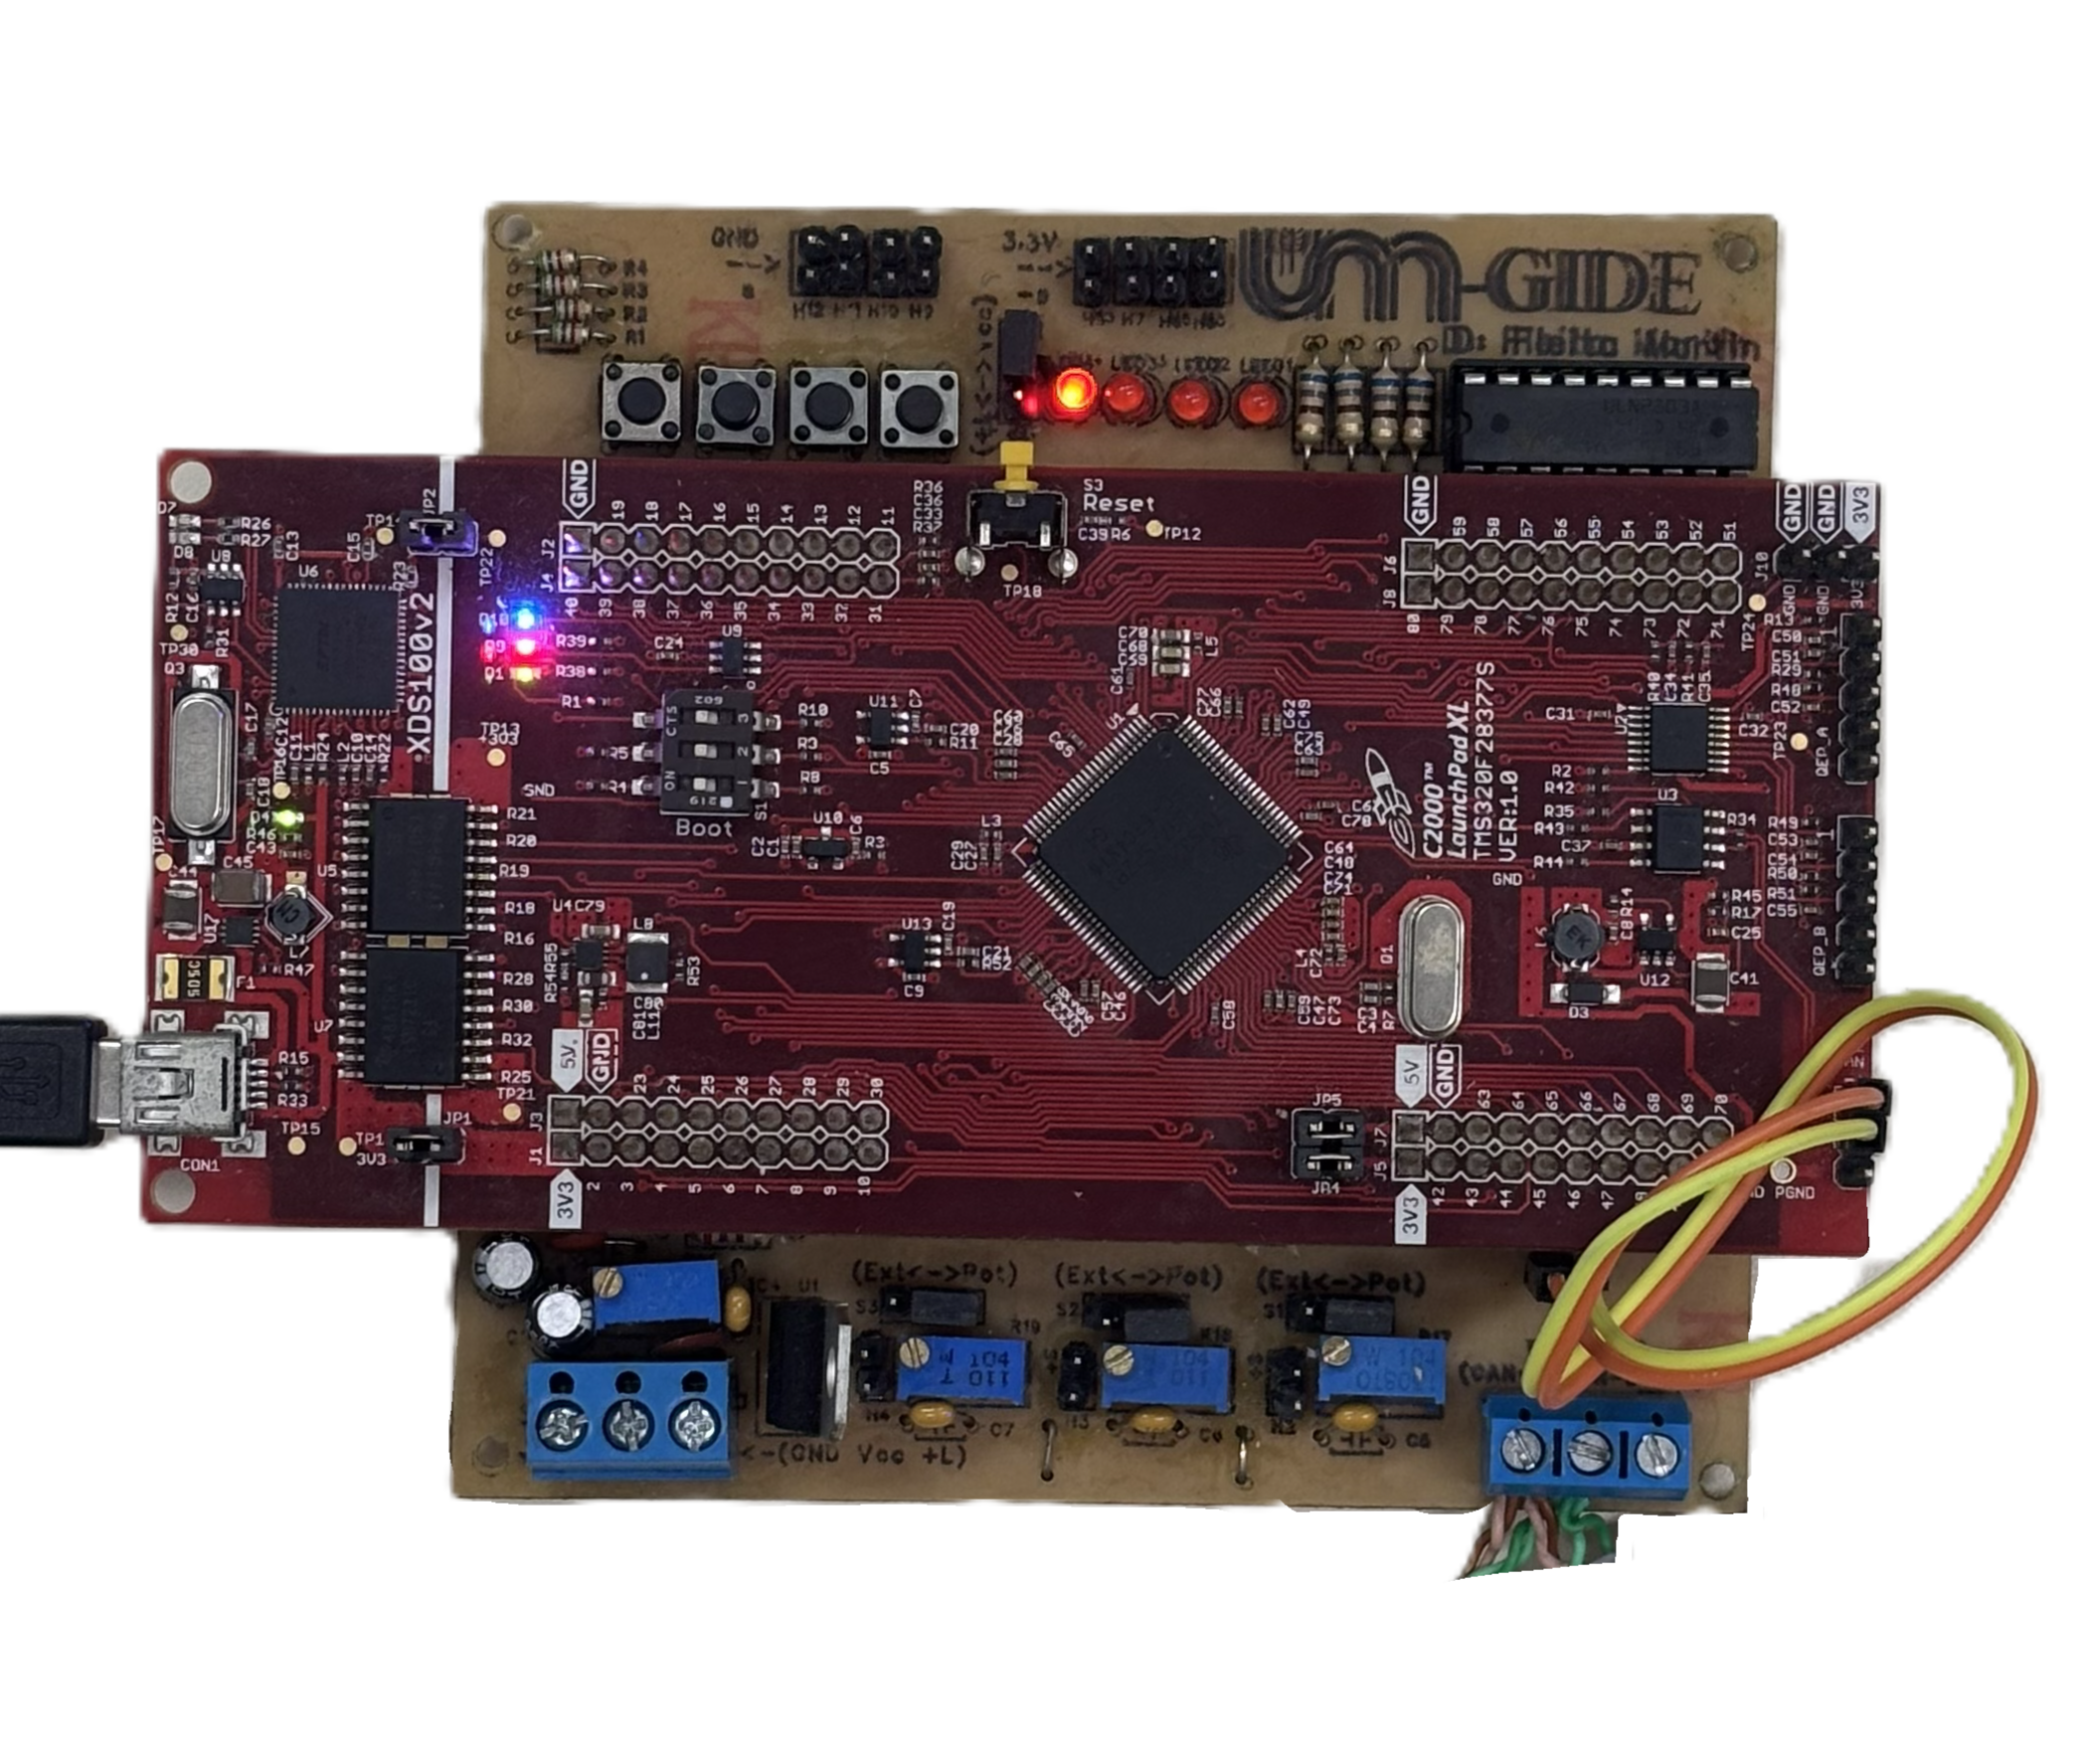
\includegraphics[width=0.4\textwidth]{imagenes/TI-prueba-CAN.png}
    \caption{Placa Texas Instruments utilizada para emular pruebas de comunicación CAN}
    \label{img:ti-can}
\end{figure}

En la configuración del ensayo, una de las placas TI asume el rol de Agente de Generación (AG). Este dispositivo inyecta en el bus CAN mensajes periódicos que simulan los valores de tensión y corriente provenientes de un arreglo fotovoltaico, permitiendo al AC calcular la disponibilidad energética sin necesidad de una fuente de energía renovable real conectada.

\section{Estructuras de Comunicación}

El correcto funcionamiento del sistema distribuido depende de la integridad de los datos intercambiados en tres niveles de red distintos. A continuación, se detallan las estructuras de los paquetes implementados para cada protocolo, especificando el formato de los datos para garantizar la interoperabilidad entre las diferentes plataformas de hardware.

\subsection{Bus CAN}
La comunicación entre el AC y el AG se realiza mediante tramas estándar CAN 2.0B. Es fundamental destacar que, para el empaquetado de los datos numéricos que ocupan más de un byte, se utiliza el formato Little Endian. Esto significa que el byte menos significativo (LSB) se transmite primero, seguido por el byte más significativo (MSB). Esta convención debe ser respetada rigurosamente por ambos microcontroladores para una correcta reconstrucción de los valores enviados en 16 bits.

La Tabla~\ref{tab:paquetes_can} detalla los identificadores (ID) y la codificación de los datos físicos utilizados en el ensayo. Los valores de tensión y corriente se envían como enteros sin signo.

\begin{table}[ht!]
\centering
\caption{Estructura de paquetes CAN para la integración con placas TI}
\label{tab:paquetes_can}
\begin{tabular}{|l|l|l|l|}
\hline
\textbf{ID CAN} & \textbf{Emisor} & \textbf{Estructura de Datos (Payload)}\\ \hline
0x610 & Agente Gen. & Byte 0-1: Tensión ($V_{fv}$) \\
      & (TI F28377S) & Byte 2-3: Corriente ($I_{fv}$) \\ \hline
0x620 & Agente Carga & Byte 0-1: Consumo Total \\ 
      & (ESP32 AC) & \\ \hline
\end{tabular}
\end{table}

\subsection{ESP-NOW}
Para la coordinación inalámbrica entre el AC y los NC's, se utilizan tramas de longitud fija que minimizan la latencia. A diferencia del bus CAN, aquí se transmiten valores en punto flotante para mayor precisión en la toma de decisiones del algoritmo distribuido. La estructura de estos mensajes se presenta en la Tabla~\ref{tab:paquetes_espnow}.

\begin{table}[ht!]
\centering
\caption{Estructura de mensajes ESP-NOW de control}
\label{tab:paquetes_espnow}
\begin{tabular}{|l|l|l|}
\hline
\textbf{Tipo} & \textbf{Emisor} & \textbf{Datos} \\ \hline
Disponibilidad & Agente Carga & \texttt{float availableCurrent} (Límite calculado) \\ \hline
Consenso & Nodo Consumo & \texttt{float current} (Consumo propio) \\
         &              & \texttt{uint8\_t priority} (Nivel 0-3) \\
         &              & \texttt{float totalCurrent} (Suma acumulada) \\ \hline
\end{tabular}
\end{table}

\subsection{MQTT}
Finalmente, para la integración con la plataforma IoT, el sistema publica la telemetría en formato JSON a través de una red TCP/IP. Este formato es ideal para la interoperabilidad con sistemas web y bases de datos. La Tabla~\ref{tab:topicos_mqtt} describe la organización jerárquica de los tópicos a los que se suscribe el servidor, definiendo la frecuencia de actualización para cada tipo de dato.

\begin{table}[ht!]
\centering
\caption{Organización de Tópicos MQTT y frecuencia de publicación}
\label{tab:topicos_mqtt}
\begin{tabular}{|l|l|l|}
\hline
\textbf{Tipo de dato} & \textbf{Tópico MQTT} & \textbf{Descripción} \\ \hline
Datos por nodo & \texttt{nodo/<ID>} & Publica el consumo instantáneo individual. \\ \hline
Totales sistema & \texttt{energia/totales} & Publica las variables globales del sistema. \\ \hline
Heartbeat & \texttt{status} & Notificación periódica de estado de conexion\\ 
         &              &  del AC al broker. \\ \hline
\end{tabular}
\end{table}

Las cargas útiles (payloads) de los mensajes están estructuradas como objetos JSON estándar. La Tabla~\ref{tab:payload_nodo} muestra el formato utilizado para reportar la actividad de cada nodo individual, mientras que la Tabla~\ref{tab:payload_total} detalla el mensaje consolidado que describe el estado general de la microrred.

\begin{table}[ht!]
\centering
\caption{Payload JSON: Datos por Nodo}
\label{tab:payload_nodo}
\begin{tabular}{|l|l|l|}
\hline
\textbf{Campo} & \textbf{Tipo} & \textbf{Descripción} \\ \hline
\texttt{nodo} & string & Identificador único del nodo (ej: ``nodo\_1'') \\ \hline
\texttt{consumo} & float & Consumo medido en Amperes o Watts \\ \hline
\texttt{fecha} & string (ISO) & Marca de tiempo (ej: ``2025-02-18T14:55:10'') \\ \hline
\end{tabular}
\end{table}

\begin{table}[ht!]
\centering
\caption{Payload JSON: Datos Totales del Sistema}
\label{tab:payload_total}
\begin{tabular}{|l|l|l|}
\hline
\textbf{Campo} & \textbf{Tipo} & \textbf{Descripción} \\ \hline
\texttt{potencia} & float & Potencia total instantánea disponible \\ \hline
\texttt{corriente} & float & Corriente total disponible \\ \hline
\texttt{tension} & float & Tensión eficaz de red medida \\ \hline
\texttt{consumo\_total} & float & Sumatoria del consumo de todos los NC's \\ \hline
\texttt{fecha} & string (ISO) & Marca de tiempo sincronizada \\ \hline
\end{tabular}
\end{table}

\section{Validación Experimental}

Para evaluar la respuesta del algoritmo de priorización ante escenarios de generación variable, se diseñó un ensayo dinámico integral. Se conectaron cargas reales a los NC's, tal como se muestra en la Figura~\ref{img:prueba-carga}, configurando un escenario con diferentes tipos de demanda y niveles de importancia:

\begin{figure}[hbt!]
    \centering
    \includegraphics[width=0.7\textwidth]{imagenes/prueba-carga.jpg}
    \caption{Conexión de cargas para ensayo de la gestión del consumo}
    \label{img:prueba-carga}
\end{figure}

\begin{itemize}
    \item \textbf{NC2 (Crítica - Prioridad 0):} Se utilizó una carga resistiva de alta potencia simulada mediante un banco de resistencias con dos niveles de operación (4 A y 8 A), representando equipos esenciales que no deben salir de servicio.
    \item \textbf{NC3 (Prioridad Alta - Prioridad 1):} Se conectó una pava eléctrica, representando una carga resistiva de uso intermitente pero importante.
    \item \textbf{NC4 (Prioridad Baja - Prioridad 3):} Se empleó un banco de lámparas incandescentes, simulando iluminación o cargas prescindibles que pueden ser desconectadas en primer lugar.
\end{itemize}

La condición de entrada para el ensayo fue un perfil de irradiancia solar simulado. En la placa TI que actúa como Agente de Generación, se programó una curva de generación que emula el comportamiento de un día solar completo (amanecer, mediodía, atardecer), pero comprimido temporalmente en un ciclo acelerado de 5 minutos. Esto permitió someter al sistema a rampas pronunciadas de subida y bajada de disponibilidad energética, forzando la actuación de los NC y validando la respuesta del algoritmo.

\subsection{Análisis de Resultados}

La Figura~\ref{img:validacion} presenta la evolución temporal de las corrientes durante el ensayo completo. La línea punteada verde representa la corriente disponible ($I_{disp}$) dictada por el perfil solar simulado, mientras que la línea punteada roja muestra el consumo total ($I_{total}$) agregado de la red que el sistema intenta regular.

\begin{figure}[hbt!]
    \centering
    \includegraphics[width=1\textwidth]{imagenes/prueba.png}
    \caption{Resultados del ensayo de la gestión de consumos bajo perfil de irradiancia simulado}
    \label{img:validacion}
\end{figure}

El comportamiento del sistema se analiza cronológicamente a través de los eventos marcados en la gráfica, demostrando la capacidad de auto-regulación de los NC's:

\begin{itemize}
    \item \textbf{Inicio (Instantes 0-1):} Con una disponibilidad inicial baja pero suficiente, se conecta manualmente la carga crítica (NC2). El sistema detecta que hay margen operativo y permite su funcionamiento continuo sin restricciones.
    \item \textbf{Aumento de Generación (Instantes 2-3):} A medida que la irradiancia simulada aumenta hacia el mediodía, crece la capacidad de corriente disponible. Esto habilita la conexión manual de cargas adicionales. Primero se conecta el banco de lámparas (NC4, prioridad baja) y posteriormente la pava eléctrica (NC3, prioridad alta). En esta fase, el sistema admite todas las cargas por un momento debido al periodo de estabilizacion de las cargas y proceso de consenso entre los NC.
    \item \textbf{Saturación y Desconexión (Instante 4):} Se alcanza el punto de inflexión donde el sistema reconoce que la demanda agregada supera a la disponibilidad. El algoritmo distribuido detecta inmediatamente la condición de déficit ($I_{total} > I_{disp}$). Siguiendo estrictamente la lógica de prioridades, el sistema decide automáticamente desconectar el NC4, ya que posee la prioridad más baja (P3). Esta acción estabiliza la red de forma instantánea, protegiendo a las cargas de mayor jerarquía.
    \item \textbf{Reconexión Automática (Instante 5):} Al aumentar nuevamente la disponibilidad debido al pico de mediodía simulado, el nodo desconectado (NC4) evalúa su condición de reconexión. El nodo verifica matemáticamente que existe un margen suficiente ($I_{disp} > I_{total} + I_{propia} + Margen$) y procede a reconectarse automáticamente, demostrando la capacidad del sistema para recuperar cargas cuando las condiciones energéticas mejoran.
    \item \textbf{Descenso de Generación (Instantes 6-7):} Al simular el atardecer, la disponibilidad comienza a caer. El sistema reacciona desconectando escalonadamente las cargas según su importancia. Primero se desconecta nuevamente el NC4 (baja prioridad) y, al continuar el descenso de la curva de generación, se fuerza la desconexión del NC3 (alta prioridad), preservando la energía restante exclusivamente para la carga crítica.
    \item \textbf{Colapso Simulado (Instante 8):} La generación cae por debajo del mínimo necesario incluso para sostener la carga crítica. En este punto extremo, el sistema protege la integridad de la microrred desconectando finalmente al NC2. Es interesante observar que se produce una breve reconexión del NC4; esto ocurre porque su consumo es menor que el de la carga crítica y sí encaja dentro del pequeño margen de energía remanente, lo cual valida que la decisión se basa puramente en la capacidad matemática disponible en tiempo real y no en estados predefinidos.
\end{itemize}

Este ensayo valida integralmente la lógica de control distribuido, demostrando que los NC's son capaces de auto-gestionarse para mantener el equilibrio energético de la microrred sin intervención del usuario, respetando estrictamente la jerarquía de prioridades establecida.